\section{Minh hoạ}

\begin{frame}{Minh họaquá trình sinh cử chỉ}
	\vspace{10pt}
	\begin{columns}
		\begin{column}{0.7\textwidth}
			\begin{itemize}
				\item Sinh cử chỉ (Gesture Generation) là gì?
				
				\begin{figure}[h]
					\centering
					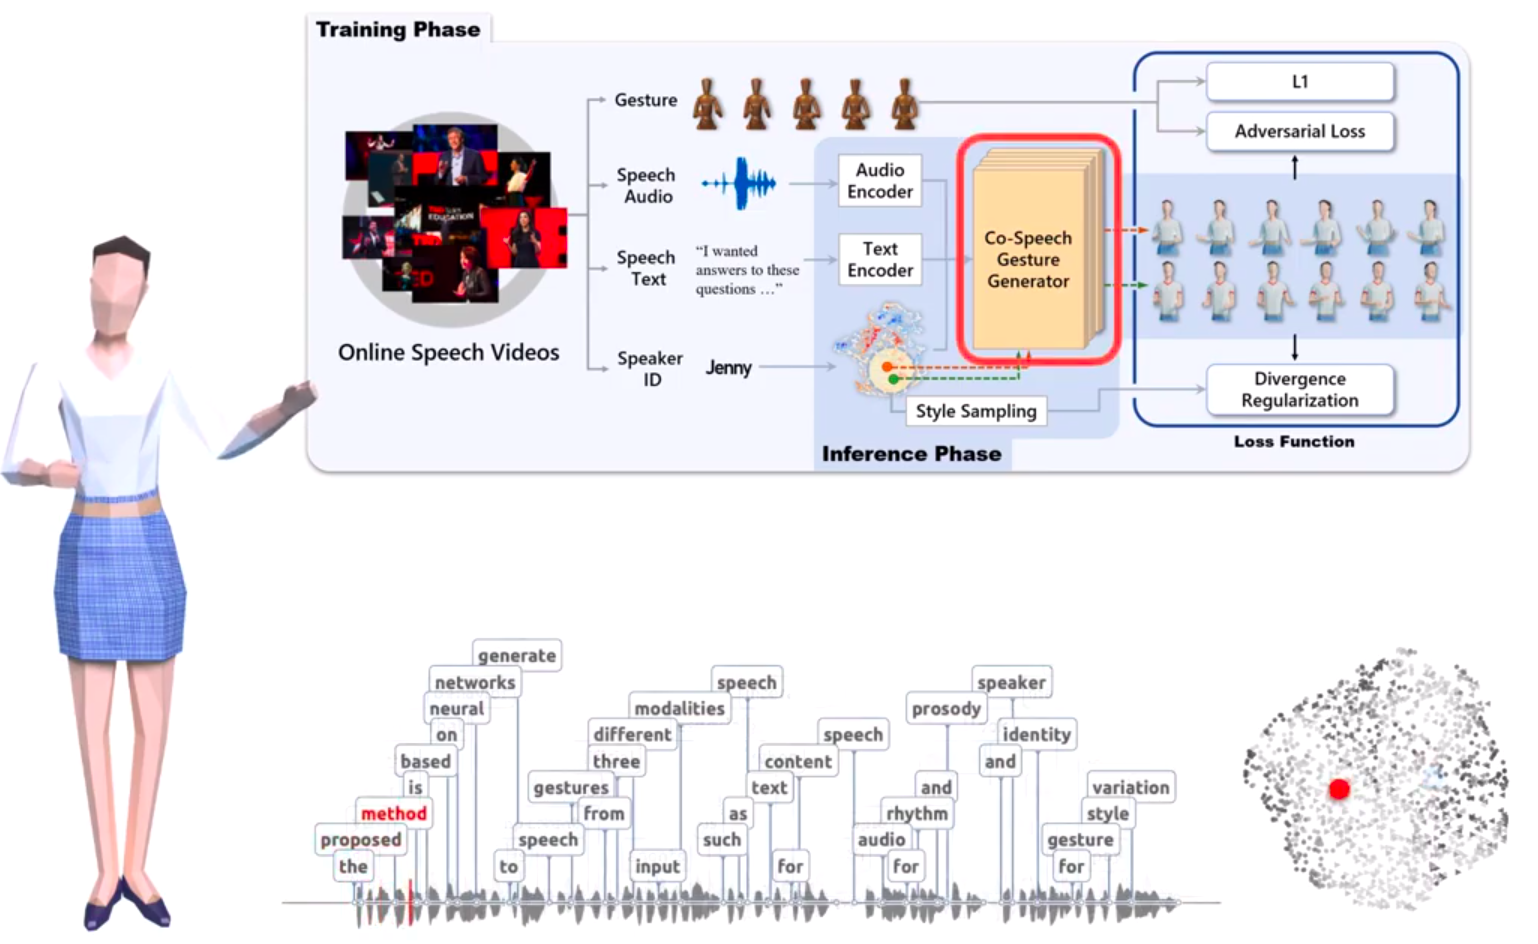
\includegraphics[width=\textwidth]{GestureGenerationExplain}
				\end{figure}
			
%				\item Mục tiêu của việc sinh cử chỉ?
%					\begin{quote}
%					"The goal of Gesture Generation is to generate gestures that are natural, realistic, and appropriate for the given context."
%				\end{quote}
			\end{itemize}
			ACM CCS: • Human-centered computing → Human computer interaction (HCI).
			
		\end{column}
		\begin{column}{0.3\textwidth} % Right column for image
			\begin{figure}[h]
			\centering
			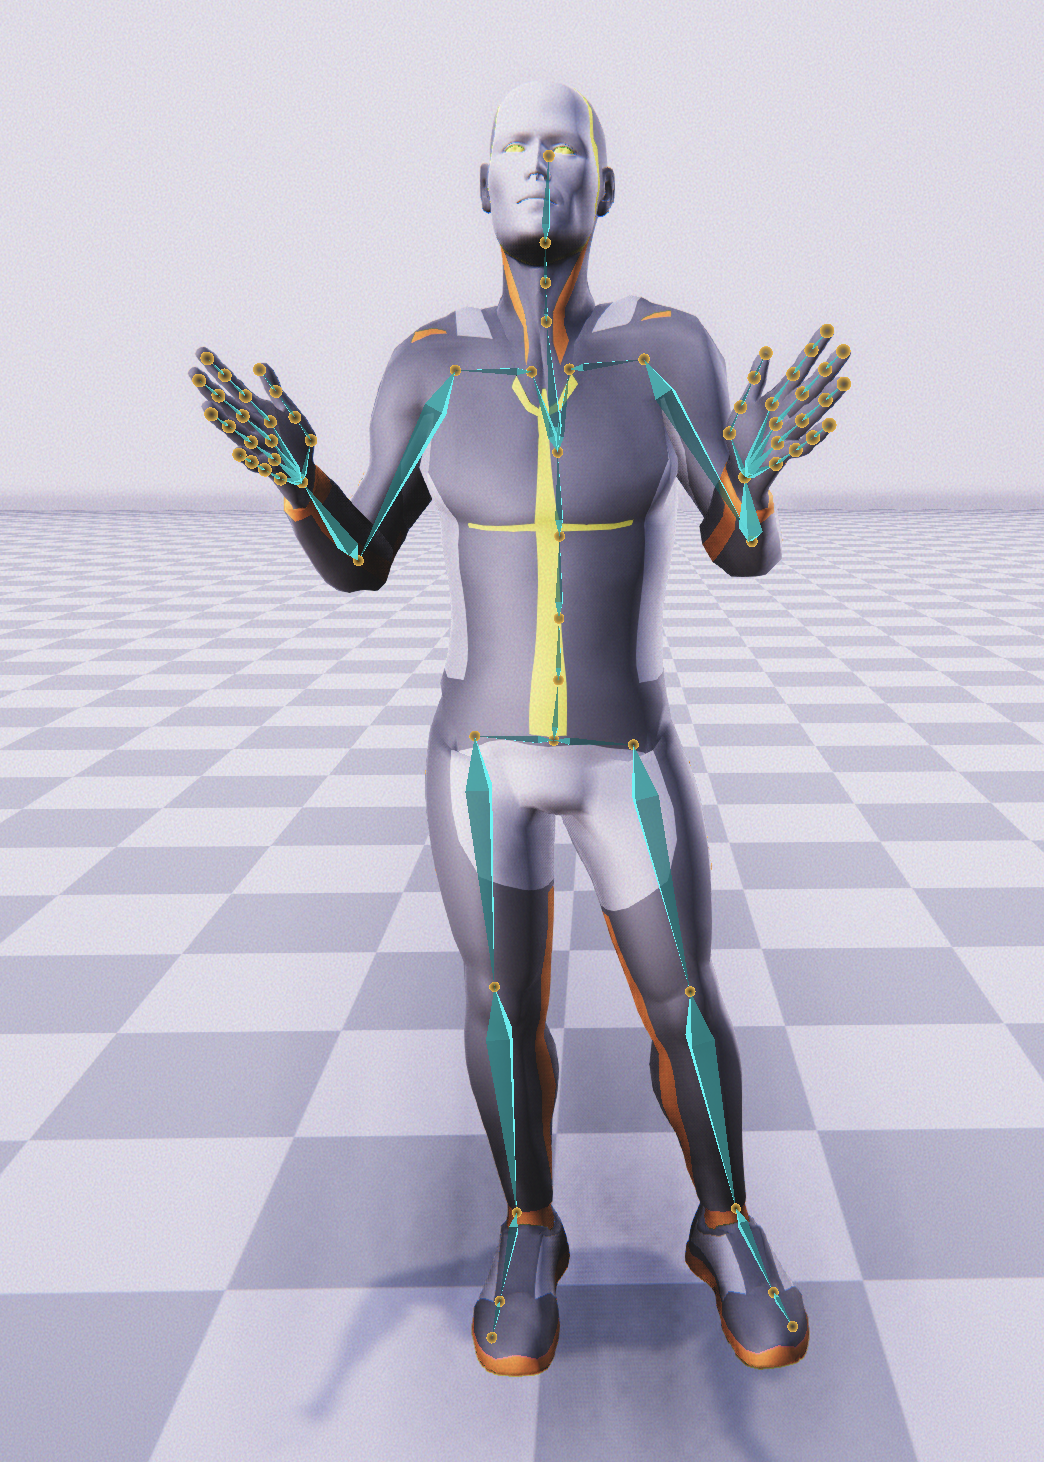
\includegraphics[height={6cm}]{SampleAnimation}
			
%				\begin{quote}
%					{\tiny
%					"Your work is gonna fill a large part of your life . And the only way to be truly satisfied is to do what you believe is great work and the only way to do great work is to love what you do."}
%				\end{quote}
				
			{
			\small Demo Gesture Generation: \href{https://www.youtube.com/watch?v=B6nv1kQmi-Q}{\textcolor{blue}{\uline{Youtube}}}
			}
			\end{figure}
		\end{column}
	\end{columns}
\end{frame}

%\begin{frame}
%\frametitle{Bulleted list}
%\begin{itemize}\itemsep=12pt
%\item XXX
%\vspace*{0.5em}
%\begin{itemize}
%\item XXX
%\item XXX
%\item XXX
%\end{itemize}
%\item XXX
%\vspace*{0.5em}
%\begin{itemize}
%\item XXX
%\item XXX
%\item XXX
%\end{itemize}
%\item XXX
%\end{itemize}
%\end{frame}

%\begin{frame}
%\frametitle{Pictures with tikz}
%\begin{center}
%\begin{tikzpicture}
%	[scale=1.5,dot/.style={circle,draw=black!100,fill=black!100,thick,inner sep=0pt,minimum size=2pt}]
%    \node[dot] at (-1,0) (n1) {};
%    \node[dot] at (0,1)  (n2) {};
%    \node[dot] at (1,0)  (n3) {};
%    \node[dot] at (0,-1) (n4) {};
%    \draw[gray] (-1.5,0) -- (1.5,0);
%    \draw[gray] (0,-1.5) -- (0,1.5);
%    \draw[black,thick] (n1) -- (n2) -- (n3) -- (n4) -- (n1) -- cycle;
%    \draw[orange,thick] (-1,0.5) -- (0,1) -- (1,1.5);
%\end{tikzpicture}
%\qquad
%\begin{tikzpicture}
%	[scale=1.5,dot/.style={circle,draw=black!100,fill=black!100,thick,inner sep=0pt,minimum size=2pt}]
%    \draw[gray] (-1.5,0) -- (1.5,0);
%    \draw[gray] (0,-1.5) -- (0,1.5);
%    \draw[black,thick] (-1,1) -- (0,0) -- (1,1);
%\end{tikzpicture}
%\end{center}
%\end{frame}


%\begin{frame}
%\frametitle{Pictures with tikz}
%\begin{itemize}\itemsep=12pt
%	\item convex envelope of (nonconvex) $f$ is the largest convex underestimator $g$
%    \item \ie, the best convex lower bound to a function
%        \vspace*{1em}
%\begin{center}
%\begin{tikzpicture}
%    \draw[gray] (-1.5,0) -- (1.5,0);
%    \draw[gray] (0,-0.5) -- (0,1.5);
%    \draw[black,thick] (-1,1) -- (0,0) -- (0.5,0.5) -- (1,-0.25) -- (2,1);
%    \draw[black,dashed] (0,0) -- (1,-0.25);
%\end{tikzpicture}
%\end{center}
%%    \item \textbf{example}: $\ell_1$ is the envelope of $\card$ (on unit $\ell_\infty$ ball)
%%    \item \textbf{example}: $\|\cdot\|_*$ is the envelope of $\rank$ (on unit spectral norm ball)
%%    \item various characterizations: \eg, $f^{**}$ or convex hull of epigraph
%\end{itemize}
%\end{frame}